\documentclass[12pt,oneside,justify]{book}

\usepackage[utf8]{inputenc}
\usepackage{mathptmx}
\usepackage{geometry}
\usepackage{fancyhdr}
\usepackage{tocloft}
\usepackage{titlesec}
\usepackage{textcomp}
\usepackage{pdfpages} 
\usepackage{graphicx}
%\usepackage[none]{hyphenat}
\usepackage[magyar]{babel}
\graphicspath{ {images/} }
\usepackage[
backend=biber,
]{biblatex}  % irodalomjegyzék

\titleformat{\chapter}{\normalfont\huge}{\thechapter.}{20pt}{\huge} % egyedi chapter szöveg

\geometry{
	a4paper,
	lmargin=3cm,
	tmargin=3cm,
	bmargin=3cm,
	rmargin=2cm
}

\fancyhead
\fancyfoot
\pagestyle{plain} % oldalstílus
\pagenumbering{arabic} % oldalszámozás 

\renewcommand{\headrulewidth}{0pt}
\renewcommand{\contentsname}{Tartalomjegyzék} % tartalomjegyzék átnevezés
\renewcommand{\listfigurename}{Ábrajegyzék} % ábrajegyzék átnevezés
\renewcommand\cftchapaftersnum{.} % chapter szám utáni pont
\renewcommand\cftchapdotsep{\cftdotsep} % chapter, és irodalomjegyzék szöveg utáni pontok
\newcommand{\sectionbreak}{\clearpage} % címsorok új oldalon

\addbibresource{bibliography.bib}

% help section - to be deleted

% \chapter{Második bekezdés}
% \section{másik bekezdés 2 szintű}
% \subsection{First Subsection}
% \paragraph{az}

% Ezt idéztem \cite{AzureFundamentals}

% \noindent // bekezdés első sorának  nem indentálása

% end help section

\begin{document} 

\includepdf{outer_cover.pdf}
\includepdf{inner_cover.pdf}

\tableofcontents

\chapter{Virtualizációról}
A számítógépek már a kezdetekben is annyira erősek voltak, hogy az átlagos felhasználási módokkal nem lehetett telljesen kiaknázni a számítási telljesítményt, vagy a tárkapacitást.
Ennek a problémakörnek a megoldására az igény az 1960-as évek közepén kezdett megnövekedni. 
Az akkori rendszerek single user, single application módban voltak képesek működni. 
Ez annyit tett, hogy a felhasználónak, ha egyszerre több folyamat futtatására volt szüksége, akkor annyi számítógépet kellett üzemeltetnie. 
A két éllovas az MIT és az IBM volt, az első kész megoldást azonban az IBM szállította. 
Az MIT-n akkor nem jól mérték fel a feladat jelentőségét, így nem szenteltek neki kellő figyelmet és elvesztették vezető szerepüket. 
Az IBM megoldásában egy specializált mainframe rendszert használtak, ahol a felhasználók párhuzamosan tudták futtatni a saját programjaikat.
A felügyeletre pedig egy parancssor állt rendelkezésre.
Ez azért volt nagy előre lépés, mert így a felhasználók egymástóll elszeparált módon dolgozhattak.
Ez volt az első lépcső a virtualizáció mai formálya felé.

A virtualizáció nem csupán az optimálisabb erőforrás elosztáshoz volt szükséges. 
A minden folyamatra külön kiszolgáló fenntartása komoly feladatok elé állította az üzemeltetésüket végzőket. 
A szerverek magas száma miatt nagy méretű adaközpontokat kellett építeni, amelyekben az megfelelő körülményeket fenntartani nagyon költséges. 
A sok különböző szerver üzemeltetése, adminisztatív szempontból sem kisebb feladat. 
A kezdeti rendszereket nem lehett távolról egyszerűen vezérelni. Léteztek ugyan KVM megoldások amelyekkel limitáltan el lehetett végezni a távoli vezérlés bizonyos lépéseit, de már például a telepítéshez - főleg ha annak fizikai adathordozóról kellett megtörténni - szükséges volt a személyes beavatkozás. 
A virtualizációs megoldások terjedésének köszönhetően, össze lehet fogni nagyobb csoportokba a szervereket. 
Aztán ezek felett a csoportok felett lehet definiálni az úgynevezett virtuális gépeket, amelyek osztoznak az erőforrásokon és a virtualizációs megoldástól függően akár mozoghatnak is a fizikai gépek között úgy, hogy a munkafolyamat nem szakad meg.

A fejlesztések azonban nem álltak le és megindultak a kutatások az alkalmazás virtualizáció irányába. 
Ezen irányú törekvések eredménye lett az egykori Sun Microsystems nevet viselő vállalat fejlesztése a Java. 
A Java nyelv legnagyobb előnye és egyben hátranya is, hogy bármely gépen elfut amelyen van Java Runtime Environment (JRE). 
A JRE felel azért, hogy az alkalmazások egy külön virtuális gépben fussanak az operációs rendszeren belül. 
Így az univerzális nyelven megírt alkalmazások telljesen szeparált, de előre jól tervezhető módon futnak szinte bármilyen hardveren és operációs rendszeren.

Jelenleg a virtualizációs megoldásokat már a biztonság fokozására használják, bővebben a gyártóspecifikus részben taglalom.

\section{On-Premises rendszerek}

\subsection{Microsoft Hyper-V\texttrademark}
A Microsoft Hyper-V története egészen 1997-ig nyúlik vissza, amikor is még a technológiát a Connectix nevű cég birtokolta. 
Az első verziós kiadása a Virtual PC-nek még Macintosh platformra készült el. 
Ezt követte 2001-ben az első Windowsos megjelenés. 
A Microsoft miután egyértelművé vált, hogy az üzleti felhasználóknak szükségük van virtualizációs megoldásokra 2003-ban megvásárolta a Virtual PC-t és az akkor még nem kiadott Virtual Servert a Connectix-től. 
A microsoft folytatta mindkét termék fejlesztését. A Virtual PC több frissítésen is átesett mígnem a Hyper-V lenem váltotta 2008-ban. 
A Virtual Server a kezdetektől fogva a szerver operiációs rendszerek és az üzleti felhasználók igényeinek megfelelően lett fejlesztve. 
Olyan nem elhanyagolható különbségekkel, hogy a szerver verzión már a kezdetektől fogva az NTFS akkori szabványának megfelelő 2TB-os méretet ki lehetett használni, míg a Virtual PC-n 127GB volt a maximum. 
A 127GB-os limit a korabeli merevlemezek kialakításából adódott, hiszen a konszumer lemezekben nem volt kontroller így az operációs rendszer nem cellák alapján címezte a lemezt hanem a geometriáját felhasználva térben írta le a helyet, ezt kellett használnia a virtuális lemezeknél is a VPC-nek, hogy az operációs rendszerek működőképesek maradhassanak.

A Microsoft Hyper-V ezzen a néven először a Windows Server 2008 operációs rendszerben debütált. 
Megjelent belőle ugyanekkor egy ingyenes verzió is Hyper-V Server néven, amely nem volt más mint egy Windows Server 2008 Core edition, a Hyper-V role-al előtelepítve, míg a többi Role letiltásra került.
A Hyper-V most már minden mai Windows kiadásban rendelkezésre áll. A kezdeti limitált képességeit az újabb verziókkal kibővítette és most már telljesen valós opció a többi nagy virtualizációs platform mellett. 

A későbbiekben bemutatom azon funkcióit amelyek a virtualizált rendszereknél elengedhetelenek és amelyeknek köszönhetően a stabilitás, biztonság, és a skálázhatóság megoldható a Microsoft saját rendszerével annélkül, hogy megvásárolható opció lenne, mint más gyártóknál.

\subsection{Nano Server}
A Windows Server 2016-os kiadásával debütált, legfőbb célja a minimális overhead melletti üzemeltetés. 
Ezen kiadás telepítés utáni öszemérete 800 megabájt, grafikus felhasználói felülete nincs így távoli managementre lett tervezve.
A kis mérete miatt nagyon gyorsan telepíthető, kevesebbszer kell Patchelni a szokásos havi iterációk helyett negyedéves ütemezéssel. 
Ezzel a rendelkezésre állása megnőtt. 
Ugyan korlátozott funkciókra használható, de azokon a területeken nagyon fontos előrelépés. 
Nano Server lehet 
\begin{itemize}
	\item Compute Node egy clusterben
	\item Scale-Out file serverben Storage Host
	\item DNS szerver
	\item IIS Webszerver
	\item Containerben futó alkalmazás gazdagép
\end{itemize}

\subsubsection{Deduplikáció}
A Microsoft a Windows Server 2012 szerver verzióban jelentette be a Deduplikációt. 
A deduplikáció az a folyamat amely feldolgozza az engedélyezett lemezek tartalmát és egyező adatblokkokat csak egyszer tárol le. Az ismétlődő blokkok esetén már csak referenciákat hagy. 
Ezzel a megoldással nagyon jó hatásfokkal lehet tárolóhelyet megtakarítani. 
A legjobban deduplikálható adatok a Virtualised Desktop Infrastructure - későbbiekben VDI rendszerek - amelyek esetén az operációs rendszer a hozzátartoztó frissítési csomagok, a feltelepített alkalmazások alapfileai többnyire minden rendszeren megegyeznek. 
Amennyiben a virtuális gépeken nagyon kevés egyedi file és telepített alkalmazás található úgy a deduplikációs ráta elérheti akár a 90\%-ot is.

%\\TODO kifejteni képekkel

\subsubsection{Virtual Network}

%\\TODO

\subsection{VMWare ESX \textsuperscript{\textregistered}}


\subsection{Oracle\textsuperscript{\textregistered} VM}


\section{Cloud megoldások}
\subsection{Microsoft Azure}


\subsection{VMWare Cloud}


\subsection{Oracle Cloud}


\section{Platformok összehasonlítása}


\chapter{Esettanulmány}
\section{Igényfelmérés}


\section{Ajánlat}


\section{Migráció cloudba}


\chapter{Esettanulmány háttércég}

\section{Architektúra}

Architektúrális szempontból Intel alapú szervereket használtam. A fejlesztői és tesztelői környezet alapját 2 db Dell PowerEdge R710-es szerver adta. A szerverek a munka ideje alatt egyenként 2 db Intel{\textsuperscript{\textregistered}} Xeon{\textsuperscript{\textregistered}} E6545 processzorral (6 mag 12 HT szál), 96 GB DDR3 ECC RAM-al, 2x64 GB Rendszer lemezekkel illetve 2x136 GB adatlemezzel volt ellátva. A kettő szerver egy failover clusterben üzemelt. A rendszer és az adat lemezek RAID1-ben üzemeltek az adatvesztés megelőzése és a magas rendelkezésre állás biztosítása érdekében. Az adatlemezek mérete sosem volt gond a Windows Deduplikációs megoldása miatt.


A rendszereinket központilag nem menedzselt, de egységes alapkonfigurációval látjuk el annak érdekében, ha az ügyfélnek segítségre lenne szüksége. 


A megépített rendszerben használt alapkonfiguráció:
\begin{itemize}
	\item Processzor: 2 mag
	\item Memória: dinamikus memória 1 GB minimum, 2 GB induláskor, 4 GB maximum.
	\item Háttértár: 64 GB Operációs rendszer lemez, 32 GB Adat lemez
	\item Hálózati kártya: 1 DB a megrendelő rendszerinek a belső hálózatán
	\item Operációs rendszer: Windows Server 2012 R2
\end{itemize}

\subsubsection{A mester image használata}

A mester image előállítása nagyban meggyorsítja a megrendelt rendszerek üzembehelyezését. Alapvetően két nagy irányzatot lehet felismerni ezen megoldások terén. 

Az első megoldás amikor már egy telljesen kész rendszert tartalmazó de syspreppelt virtuális merevlemezt másolunk át a konténer mappájába. Majd azt a virtuális gép konfigurációjakor becsatoljuk és már indítható is rendszer. Ezek után összesen a végfelhasználó szerződést kell elfogadnunk és már használatba is vehetjük a gépünket. Amelyet át kell nevezni, be kell állítani számára a megfelelő IP konfigurációt és már át is adható a felhasználónak. 

 
% \\TODO  A két irányzat alapvető lépéseit illetve a továbbiakban szükséges folyamatokat bemutatni
\begin{figure}[t]
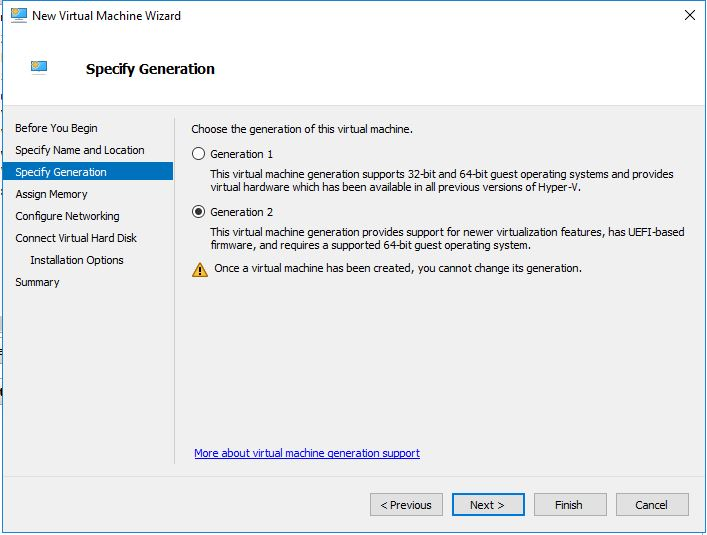
\includegraphics[width=0.8\textwidth]{generation_selection}
\caption{Generáció választás Hyper-V managerből készített virtuális gép esetén}
\label{fig:gen_selection}
\end{figure}


A másik irányzat amikor a Microsoft Deployment Toolkitet használjuk.

\section{Automatizált megoldások}


\subsection{On-prem}


Az automatizált rendszer első és lefontosabb építőköve a gyors virtális gépek elkészítése. Mivel az esettanulmányban egy szolgáltató céget tételeztem fel, így fontos volt, hogy minél kevesebb módon, lehetőleg telljesen automatikusan lehessen legyártani az igényelt virtális gépeket. 

\subsubsection{Provision-ObjectsForCompany.ps1}
Egy gyűjtő kód amely megfelelően paraméterezve elvégzni a telljes virtális gép létrehozás lépéseit. 
A következőkben taglalt scripteket hívja meg. 
A kódok végrehajtása az előkövetleményeknek megfelelően történik:
\begin{enumerate}
	\item VIrtuális Switch létrehozása ( Crete-NewVirtualSwitch.ps1 )
	\item Viruális gép(ek) létrehozása ( Create-VM.ps1 )
	\item A virtális gépek hálózatba fűzése ( Set-VMSwitchForVM.ps1 )
\end{enumerate}

% \\TODO

\subsubsection{Create-NewVirtualSwitch.ps1}

Virtuális switchek tulajdonságát korábban taglaltam. A cégnél a megrendelők rendszerei telljesen elválastott rendszerek, hacsak a megrendelők másképp nem rendelkeznek. Ellenben a virtális gépek amelyek egy megrendelőhöz kötődnek egymással közös hálózaton vannak. Szolgáltatói oldalon a cégekhez tartozó erőforrások azonosítása érdekében a megrendelő cég nevét eléfűzöm az erőforrás nevézhez. Amennyiben már létezik ilyen erőforrás úgy a script küld egy email üzenetet az üzemeltetőnek, hogy manuális ellenőrzésre van szükség.

% \\TODO ?

\subsubsection{Create-VM.ps1}

A script egy az argumentumaiban szereplő paramétereknek megfelelő VM konténert hoz létre. A beállításokat tekintve, ha valamelyik paraméter nincs felülbírálva az argumentumokban, akkor a korábban már taglalt alapbeállítás kerül felhasználásra.

A script úgy lett elkészítve, hogy képes felismerni, ha valamelyik lemez VHDX állománya már létezik.


% \\TODO




\subsubsection{Post-Configuration.ps1}
% \\TODO

\subsection{Cloud}
\noindent

\chapter{PowerShell}
\section{Történelme}
% \\TODO
\section{Programozási paradigmák}
% \\TODO

\addcontentsline{toc}{chapter}{\listfigurename}
\listoffigures
\printbibliography[heading=bibintoc,title={Irodalomjegyzék}]
\end{document}
